% SPDX-FileCopyrightText: 2023 Iegor Riepin, Tom Brown
%
% SPDX-License-Identifier: CC-BY-4.0

\lipsum[1]


\subsection{Signal 1: quality of local renewable resources}

Consider a case when datacenters are located in Denmark, Germany, and Portugal (Figure \ref{fig:dashboard1}: panel a). There are three different types of renewable resources represented by the three sites, with Denmark having a good wind resource, Germany having a moderate wind and solar resources, and Portugal having a good solar resource. The quality of local renewable resources is reflected by the average annual capacity factor for onshore wind and solar PV, as shown in the panels b and c,

Panel d on Figure \ref{fig:dashboard1} shows the modelled cost-optimal capacity of renewable generators and battery storage for 24/7 matching. In the case of inflexible loads, the procurement strategy must ensure a sufficient amount of carbon-free electricity is available round-the-clock \textit{at each site}. Due to the non-dispatchable nature of renewable resources and the relatively high energy costs of battery storage, the cost-optimal portfolio is much larger than the load. To cover the 100 MW load with perfect hourly matching, the consumer would have to procure combined wind and solar PV generators of approx. 900~MW in Denmark and 1300~MW in Germany or Portugal. In each portfolio, the proportion of wind and solar PV reflects the quality of the local resources. 

In Figure \ref{fig:dashboard1}: panel d, steps on the x-axis represent increasing flexible load, allowing for a reduction in the capacity of renewable generators and battery storage necessary for 24/7 matching. By having a degree of load flexibility, a consumer can shift the load from times of scarce renewable generation to times of abundant renewable generation in the same hour, or use the excess renewable generation at one site to cover the load at another site. In other words, with load flexibility, consumer can get the most out of the clean energy resources that are available.

The breakdown of costs associated with procurement strategy that participating is shown in Figure \ref{fig:dashboard1}: panel e. The panel shows the average cost per MWh of consumption, including renewable generation costs and battery storage costs.\footnote{Here we do not consider the option of selling the excess electricity to the regional grid. Excess electricity can thus be stored in the battery, shifted in space or time with load flexibility, or curtailed.} Demand flexibility enables consumers to better match renewable generation with demand profile, reducing over-procurement and costly battery storage. The costs are reduced in all locations, and especially in locations where hourly matching is most expensive. Modelling results show the costs of 24/7 matching in Germany are at 215~\euro/MWh when there is no load flexibility, 135~\euro/MWh when there is 10\% flexible loads, and as reduced up to 137~\euro/MWh when there is 40\% of flexible loads.

Figure \ref{fig:dashboard1}: panel f displays the total annual costs for achieving 24/7 matching at all locations (left y-axis) and their relative representation as a percentage of the inflexible scenario costs (right y-axis). The panel summarises the model results: as demand flexibility increases, 24/7 matching becomes more resoure-efficient and affordable. The value of additional flexibility also diminishes as the number of flexible loads increases, i.e., the first 10\% of flexible loads can reduce costs more than the next 10\%. A generalization of this result is presented in Section \ref{ssec:section4}.

\begin{figure*}
    \centering
    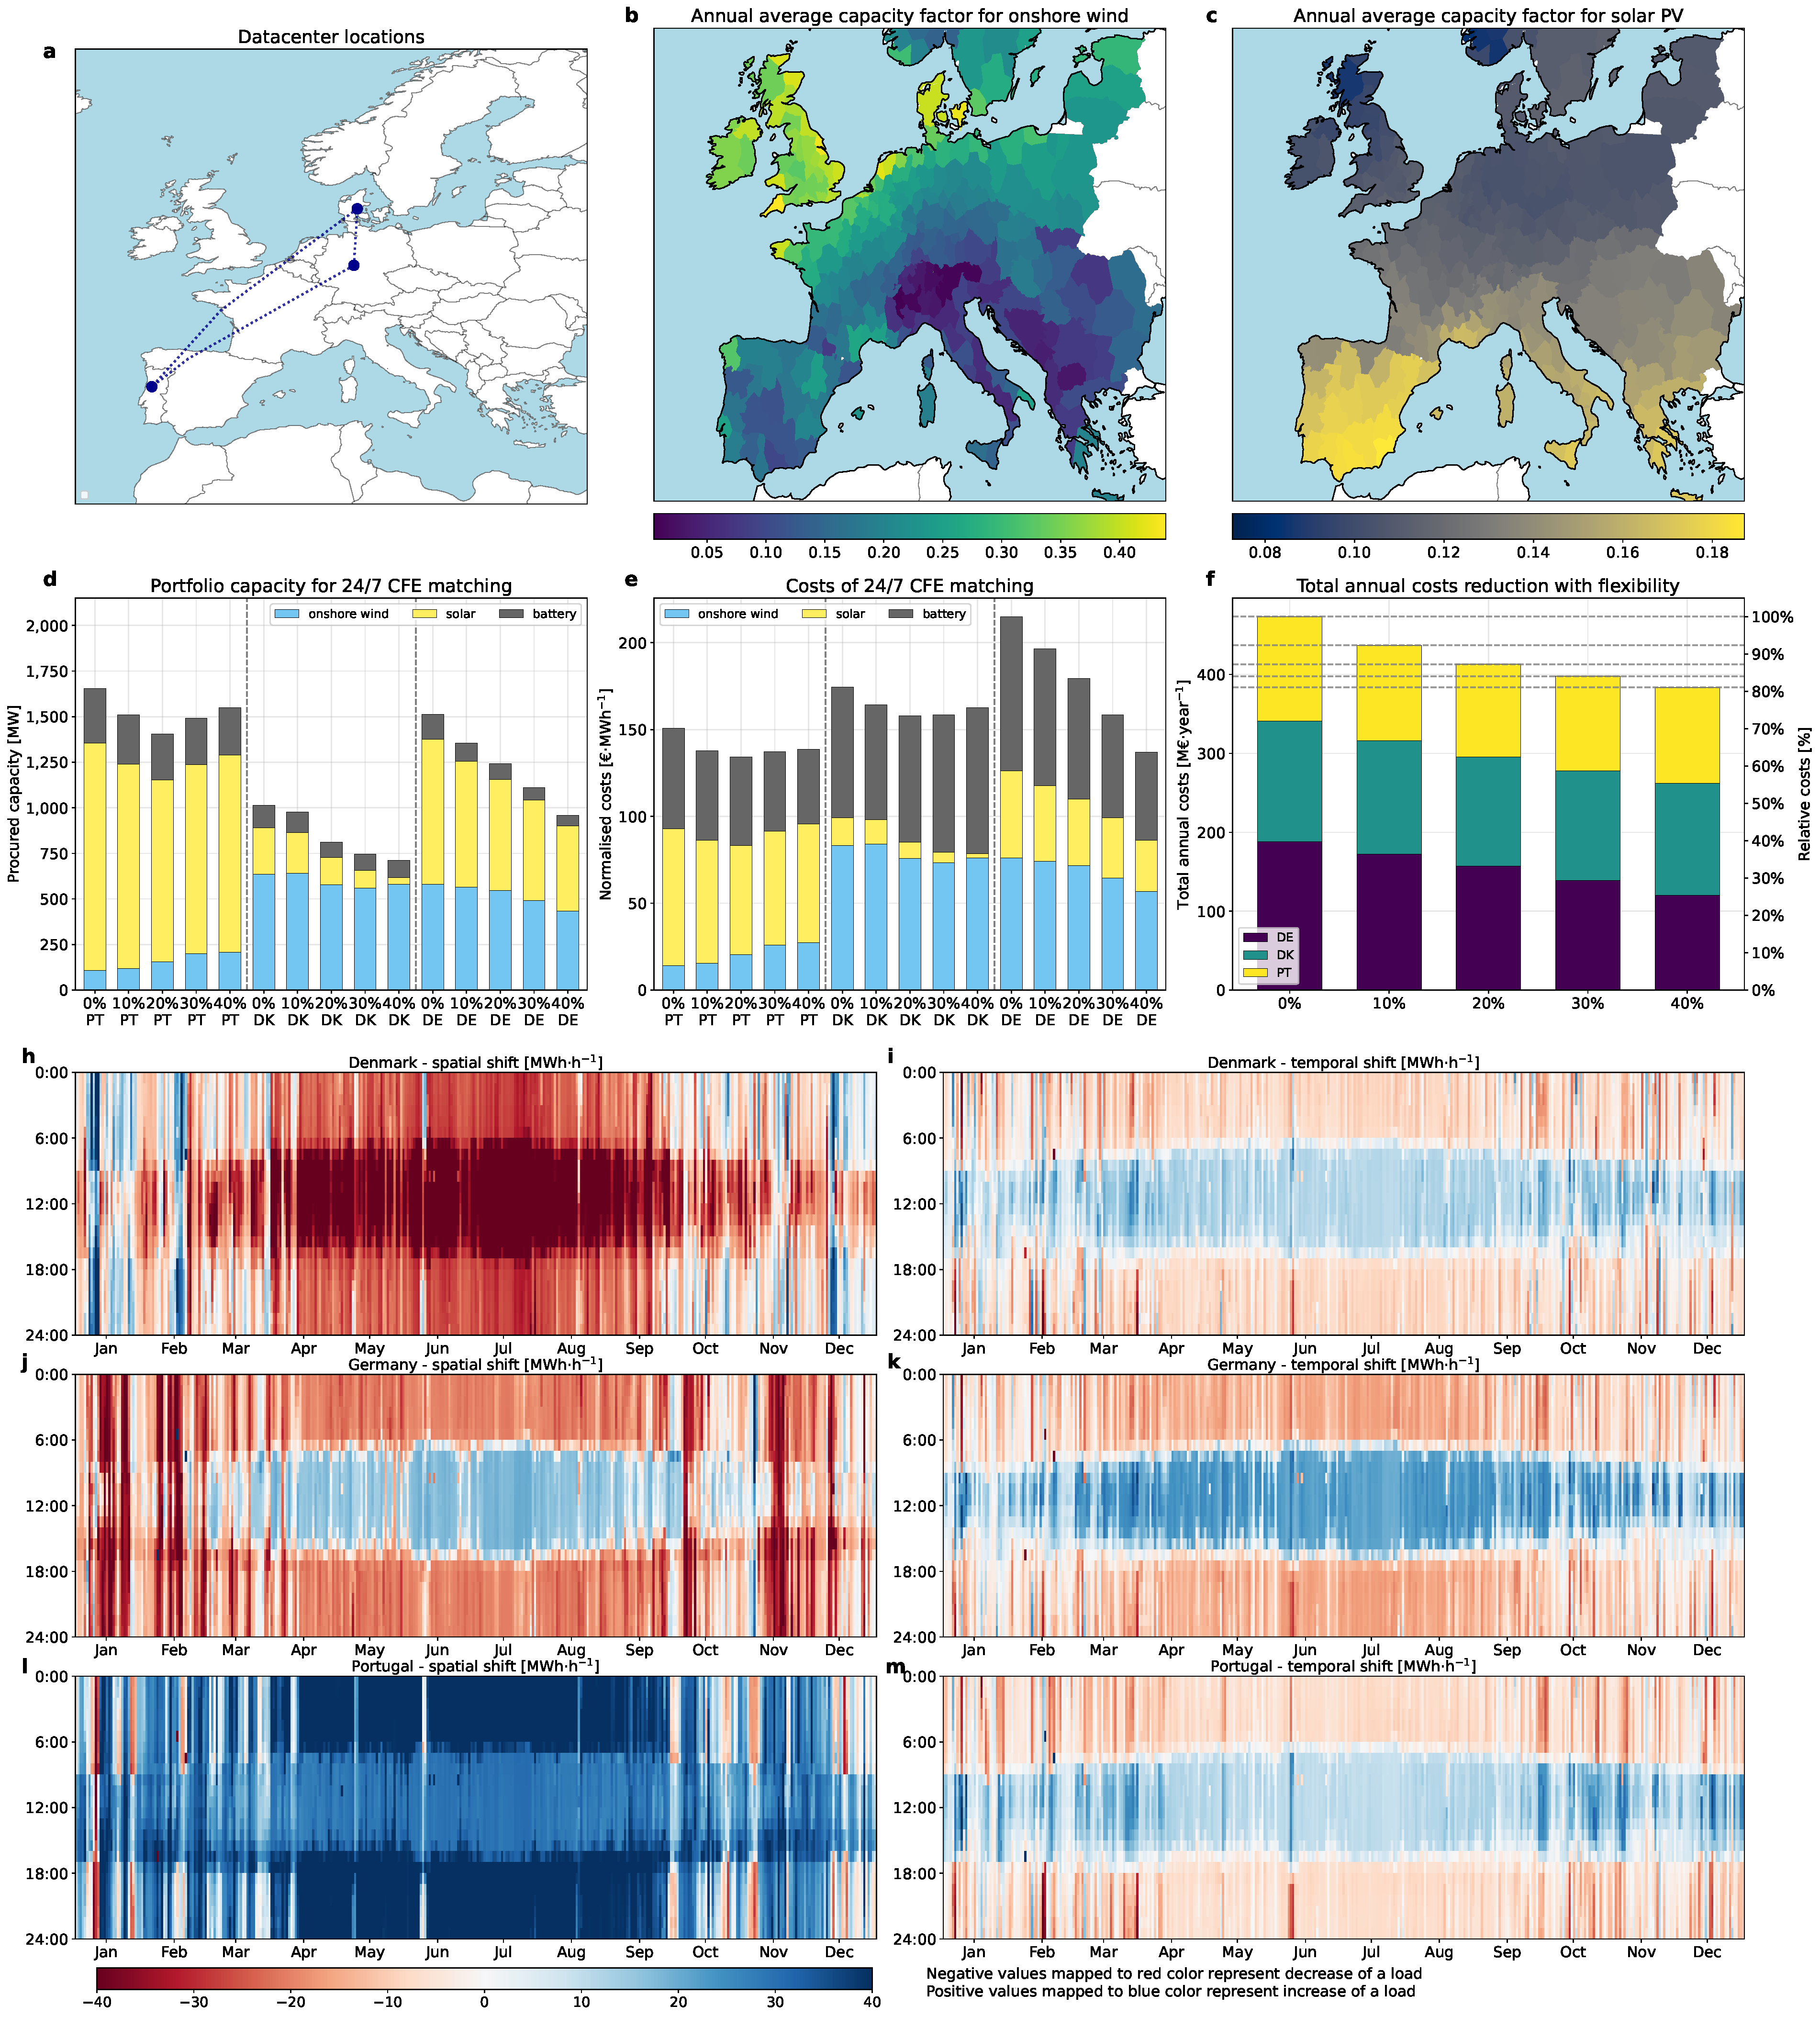
\includegraphics[width=\textwidth]{img/dashboard.pdf}
    \caption{Illustration of the signal 1: quality of local renewable resources.
        \textbf{a:} Assumed datacenter locations: Denmark, Germany, Portugal.
        \textbf{b,c:} Annual average capacity factor of onshore wind and solar photovoltaic. Data is simulated using the ERA5 reanalysis dataset for weather year 2013 and aggregated to 256 regions in Europe.
        \textbf{d:} Cost-optimal portfolio of renewable resources and battery storage sufficient for 24/7 matching. Steps on x-axis represent increasing share of flexible load.
        \textbf{e:} Cost breakdown of 24/7 matching strategy.
        \textbf{f:} Total annual costs of 24/7 matching strategy as a function load flexibility. Relative axis is normalized to the costs of inflexible load.
        \textbf{h,j,l:} Hourly spatial load shifts for the three datacenter locations. Color mapping represents the quantity of load \enquote{received} from other locations or \enquote{sent} away.
        \textbf{i,k,m:} Hourly temporal load shifts for the three datacenter locations. Color mapping represents the quantity of load shifted to a given hour from other times, or shifted from a given hour to another time.}
    \label{fig: dashboard1}
\end{figure*}


\subsection{Signal 2: low correlation of wind power generation over long distances}

\begin{figure*}
    \centering
    \includegraphics[width=\textwidth]{img/dashboard_2.png}
    \caption{Illustration of the signal 2: low correlation of wind power generation over long distances.
    \textbf{a:} Assumed datacenter locations: pairwise connections across regions with similar quality of renewable resources. Here: Ireland with Northern Ireland, or England, or the Netherlands, or Denmark (-west zone).
    \textbf{b,c:} Peason correlation of hourly capacity factor for onshore wind generation, if Denmark (-west zone, panel b) or selected region of Ireland (panel c) are taken as basis. As a result of different weather conditions, wind feed-in has a noticeable correlation falloff over distances of 300-400 km. Data is simulated using the ERA5 reanalysis dataset for weather year 2013 and aggregated to 256 regions in Europe.
    \textbf{d} Hourly spatial load shifts for the selected scenario and datacenter; here datacenter is located Denmark (and another one is located Ireland). Color mapping represents the quantity of load \enquote{received} from other locations or \enquote{sent} away.
    \textbf{e} Cost savings of 24/7 matching with increasing distance between datacenters. Costs are normalized to the cost level of inflexible load.}
    \label{fig:dashboard2}
\end{figure*}


\subsection{Signal 3: time lag in solar radiation peaks due to Earth's rotation}

\begin{figure*}
    \centering
    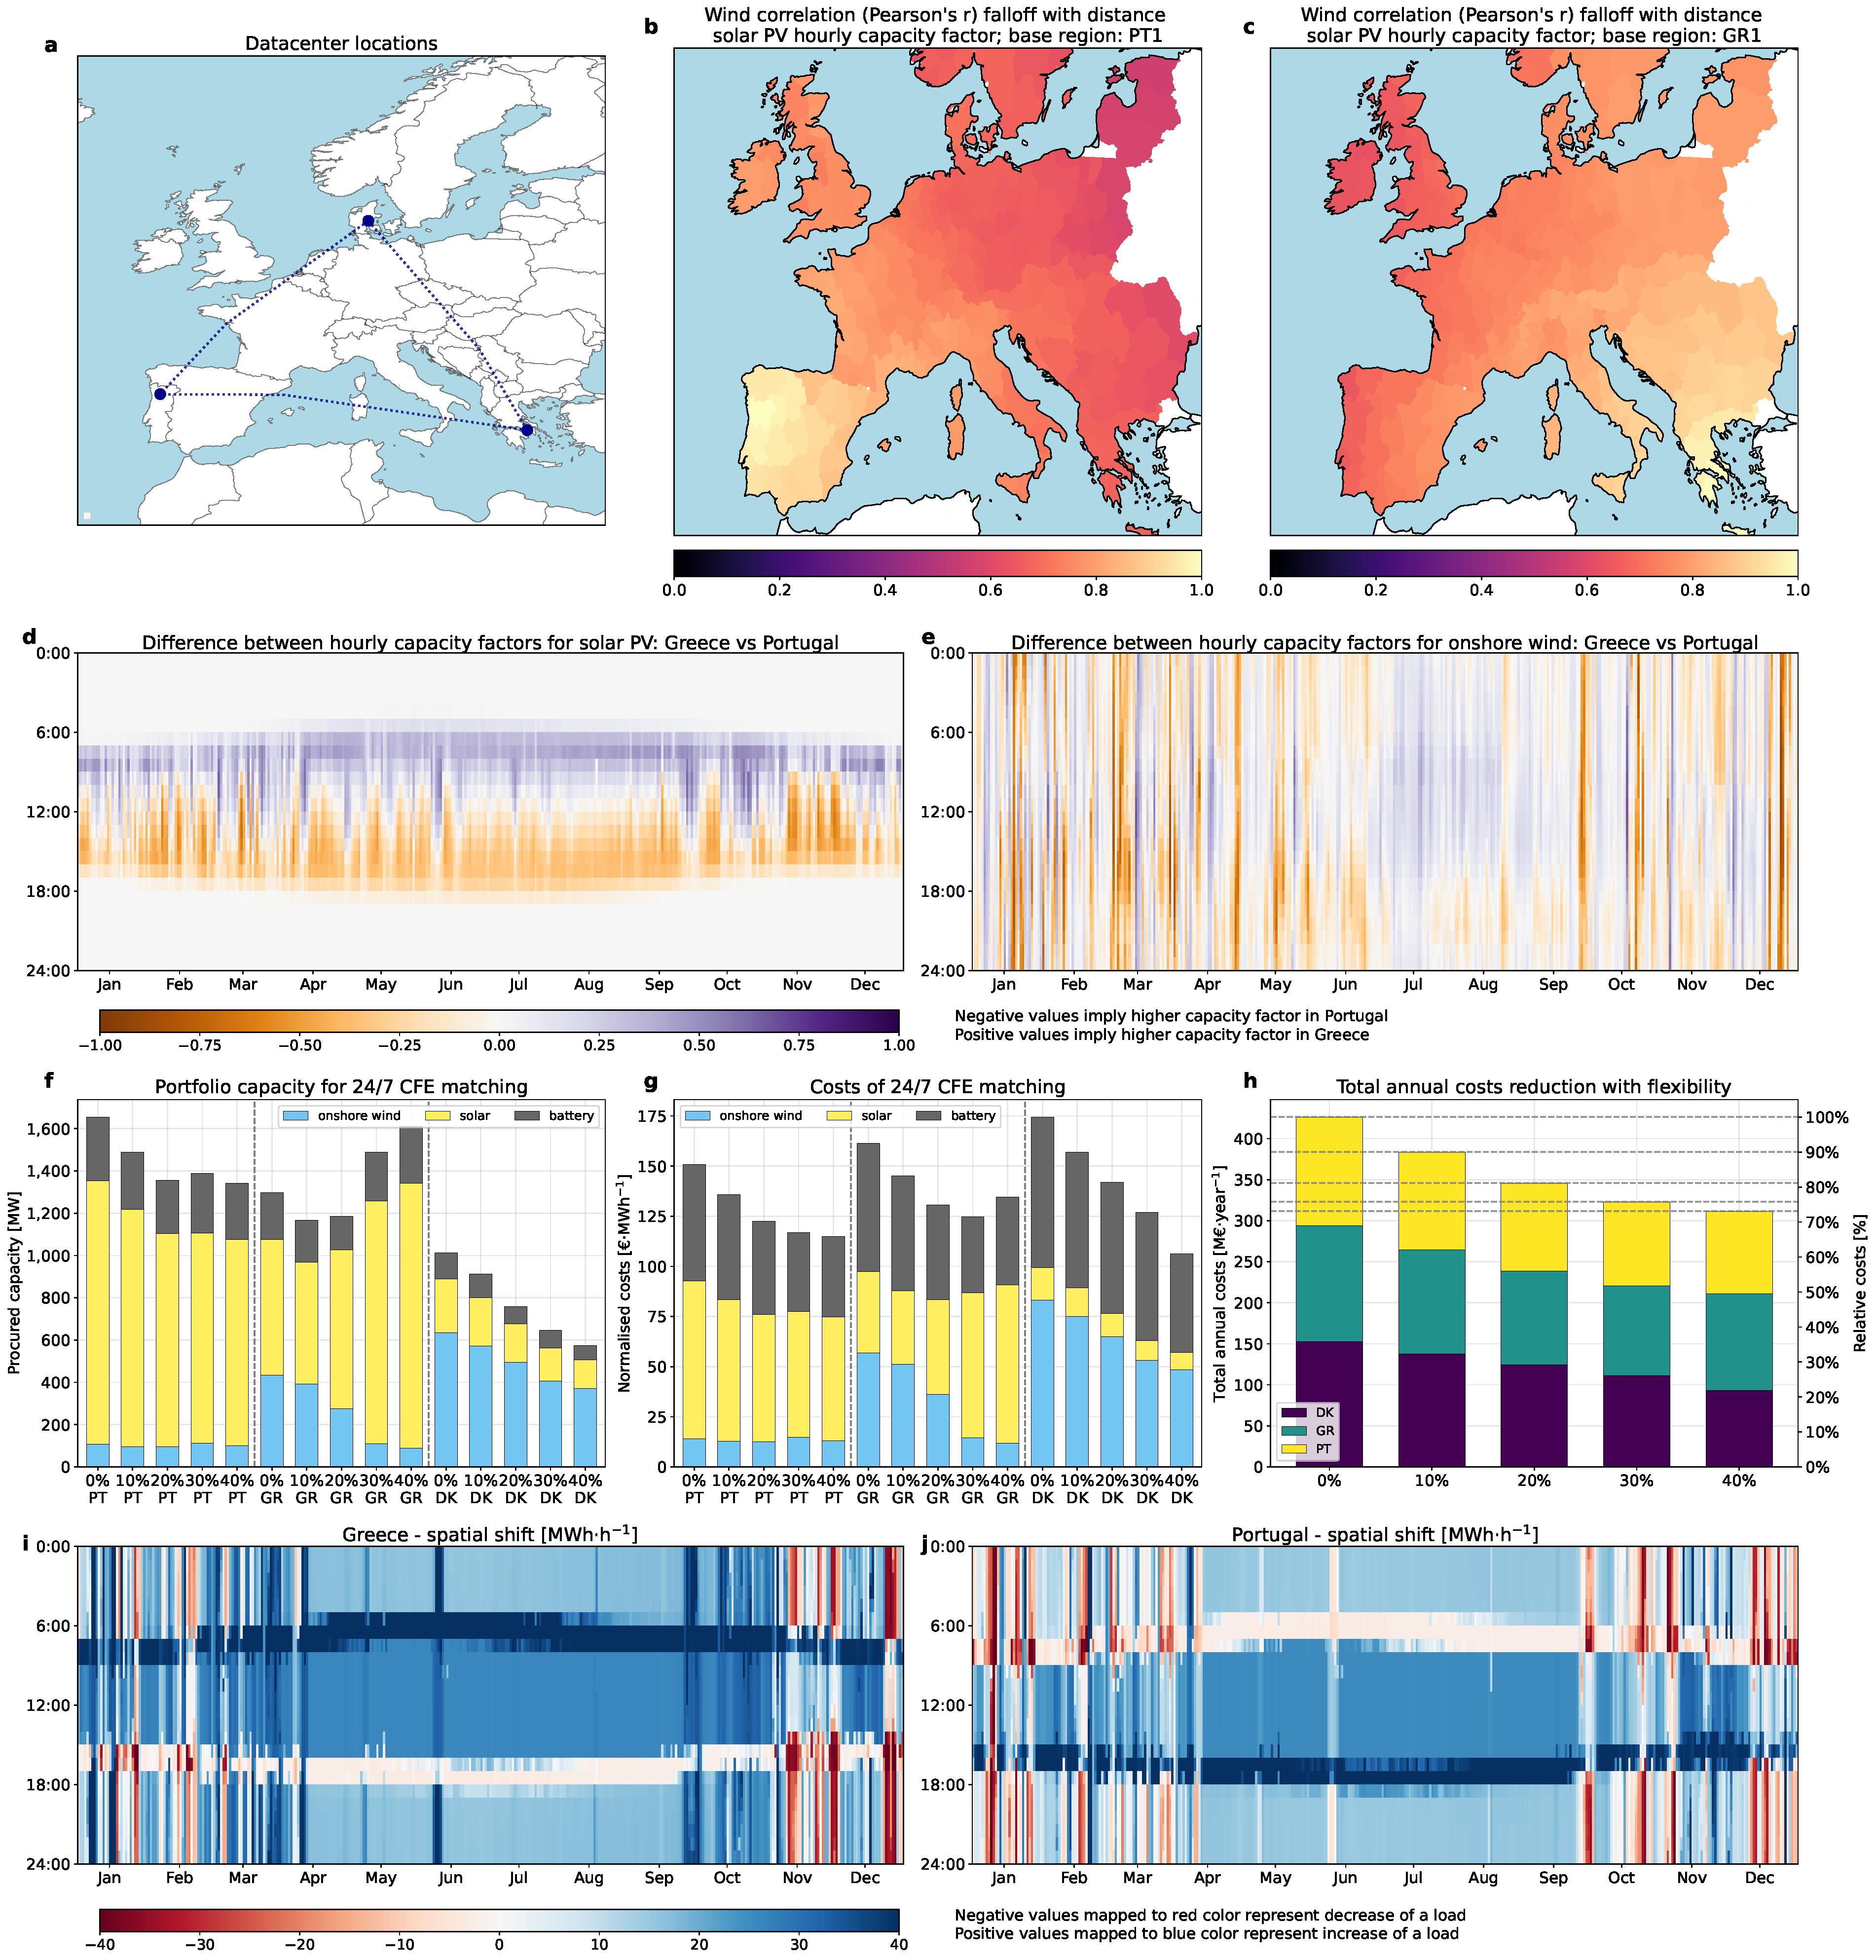
\includegraphics[width=\textwidth]{img/dashboard_3.pdf}
    \caption{Illustration of the signal 3: time lag in solar radiation peaks due to Earth's rotation.
    \textbf{a:} Assumed datacenter locations: Denmark, Portugal, Greece.
    \textbf{b,c:} Peason correlation of hourly capacity factor for solar photovoltaic generation, if selected region of Portugal (panel b) or region of Greece (panel c) is taken as basis. Solar generation remains highly correlated over long distances, in contrast to wind generation.
    \textbf{d:} Difference in solar photovoltaic hourly capacity factors between two selected locations: Greece and Portugal. The two locations are approx. 2700~km apart, which results in a noticeable lag in solar generation peaks due to Earth's rotation.
    \textbf{e:} Difference in wind generation hourly capacity factors between two selected locations: Greece and Portugal. As expected, low correlation of wind feed-in over long distance results in stochastic pattern.
    \textbf{f:} Cost-optimal portfolio of renewable resources and battery storage sufficient for 24/7 matching. Steps on x-axis represent increasing share of flexible load.
    \textbf{g:} Cost breakdown of 24/7 matching strategy.
    \textbf{h:} Total annual costs of 24/7 matching strategy as a function load flexibility. Relative axis is normalized to the costs of inflexible load.
    \textbf{i,j} Hourly spatial load shifts for the selected datacenter locations: Greece (panel i) and Portugal (panel j). Color mapping represents the quantity of load \enquote{received} from other locations or \enquote{sent} away.}
    \label{fig:dashboard3}
\end{figure*}

\subsection{Generalising the results beyond specific load locations}

\begin{figure}
    \centering
    \includegraphics[width=1\columnwidth]{img/flexibility_vs_normalized_costs.pdf}
    \caption{\lipsum[1]}
    \label{fig:flexcost}
\end{figure}
